\section{Risultati}
\label{sec:risultati}
In questa sezione si valuteranno le performance dell'algoritmo.
Per condurre questa analisi si è innanzitutto una mappa utilizzando il generatore
di mappe, poi utilizzata per l'analisi, è riportata in figura \ref{fig:dungeon}.
\begin{figure}[!htb]
	\centering
	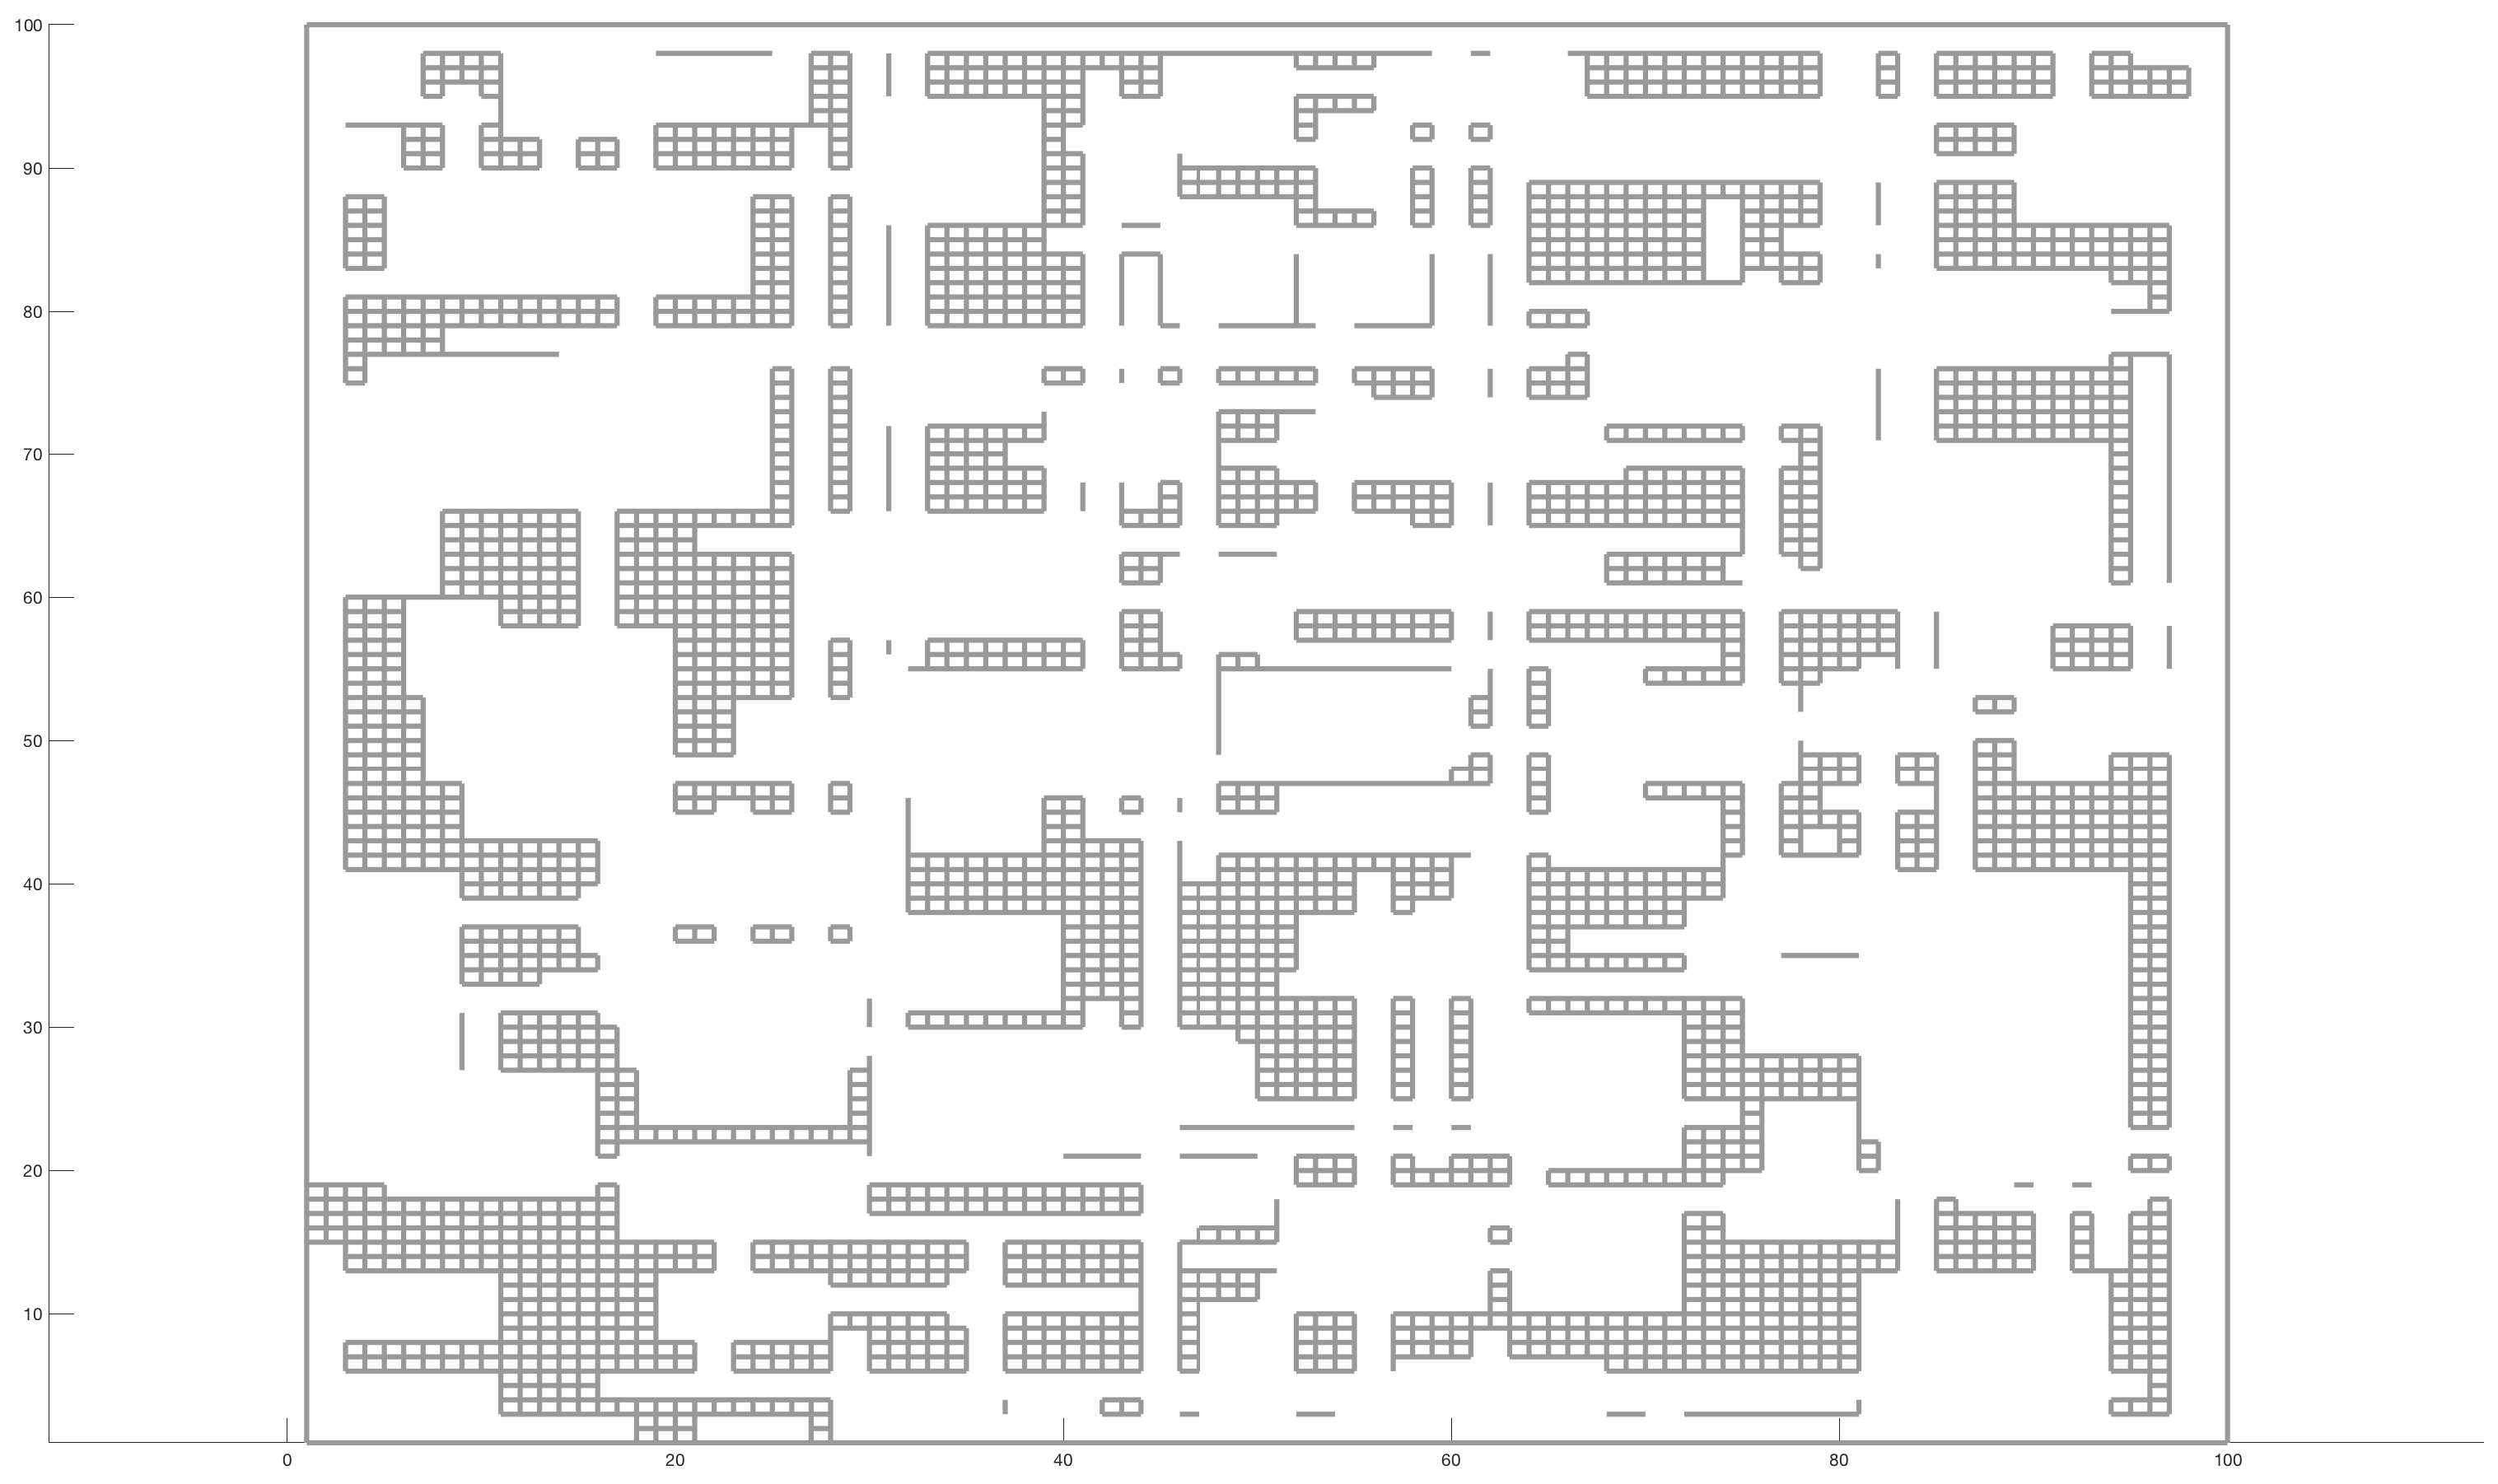
\includegraphics[width=\linewidth]{dungeon}
	\caption{esempio di scenario procedurale $40\times40$}
\label{fig:dungeon}
\end{figure}
%
Per valutare le performance si è deciso di individuare delle metriche che
permettano di saggiare il sistema.
L'obbiettivo di tale analisi è trovare il numero di robot e il tempo minimo di
simulazione che permetta di assicurare delle date performance.
La funzione di costo utilizzata è la seguente (\ref{eq:totalcost}):
\begin{equation}
	\label{eq:totalcost}
	Total_{Cost} = \alpha \cdot N +\beta \cdot T + \gamma \cdot D - \delta \cdot M
\end{equation}
$Total_{Cost}$ rappresenta la nostra funzione che vogliamo minimizzare per il
numero di robot $N$ e per il tempo di simulazione $T$. $D$ e $M$ rappresentano
invece la distanza totale percorsa dai singoli robot $(D)$, in modo da avere
anche una valutazione dei consumi richiesti, e la percentuale di mappa esplorata
$(M)$.
I coefficienti moltiplicativi ($\alpha$, $\beta$, $\gamma$, $\delta$)
rappresentano i pesi per la nostra valutazione, per esempio, se si vuol dare
maggior risalto al consumo energetico si darà maggior peso al coefficiente
$\gamma$).
Tra i vari termini che compongono la funzione una crescita dei parametri $N$,
$T$, $D$ verrà considerato un evento negativo in quanto legato a dei costi (
\begin{enumerate*}[label={\alph*)},font={\bfseries}]
\item costo nell'adozione di più robot;
\item costo in termini di efficienza energetica;
\item necessità legate ad avere nel minor tempo possibile dei risultati 
soddisfacenti
\end{enumerate*}), tutti questi termini premoltiplicati per il loro peso che ne 
definisce la loro importanza relativa aumentano la funzione di costo e per 
questo sono preceduti da un segno ``+", mentre l'esplorazione percentuale della
mappa è un dato che vogliamo che sia più alto possibile ed è per questo che 
prima del suo peso relativo $\delta $ è anticipato da un segno ``-".
Eseguendo l'algoritmo si ottengono dei risultati che nel caso dell'esplorazione
della mappa compiuta da un singolo robot fino ad un massimo di 5, inoltre oltre
a variare il numero di robot presenti con il compito di esplorare l'ambiente
sconosciuto si è fatto incrementare il tempo a disposizione dei robot per
condurre l'analisi, questo tempo (eq. (\ref{eq:totalcost}), rappresentato come
$T$) varierà da un minimo di 400 ad un massimo di 1400 secondi con incrementi di
200 secondi tra una iterazione e la successiva. Riassumendo si otterà una
tabella di valori della funzione di costo ($Total_{Cost}$) al variare del numero
di robot da 1 a 5 con incrementi di 1 e del tempo simulativo da 400 a 1400
secondi con incrementi di 200.
Una volta ottenuti i risultati viene lanciato un'algoritmo \emph{minmat} che
restituisce data una matrice in ingresso il valore dell'indice della riga e
colonna dove è presente l'elemento a valore minore nella matrice. 
I valori ottimali ottenuti sono rappresentati nella tabella
\ref{tab:optimalresults}.
È qui rappresentato un grafico che interpola i valori puntuali di $Total_{Cost}$
in una superficie in uno spazio 3D.
\begin{table}[htb]
	\centering
	\caption{Risultati ottenuti}
	\label{tab:optimalresults}
	\begin{tabular}{lcS[table-format=3.2]}
	\toprule
	\multicolumn{3}{c}{dimensioni}\\
	\midrule
      numero ottimo di robot  & [ \# ] & 3\\
      tempo ottimo di simulazione     & [\si{\second}] & 1000\\
     \bottomrule
\end{tabular}
\end{table}
